\section{Optimaler Detektor - Rauschen in digitalen Kommunikationssys. \schaum{227-9}}
\textbf{Rauschen} \textbf{verschlechtert} die \textbf{Performance}, bei \textbf{digitalen} Systemen zeigt sich dies in der
\textbf{Bitfehlerrate} $P_e$. \\
Dieses Kapitel behandelt digitale Signale, welche über einen verzerrungsfreien Kanal gesendet werden
und mit einem Additiven Weissen Gauss'schen Rauschen (AWGN) versetzt werden. 

\subsection{Binäres Übertragungssystem \schaum{226-9.2}}
Ein \textbf{binäres Signal} $s_i(t)$ \verweiskurz{09_binary_signals_error} wird
über einen verzerrungsfreien (auch ohne Intersymbol Interferenz) Kanal gesendet. \\
\begin{minipage}{10cm}
 	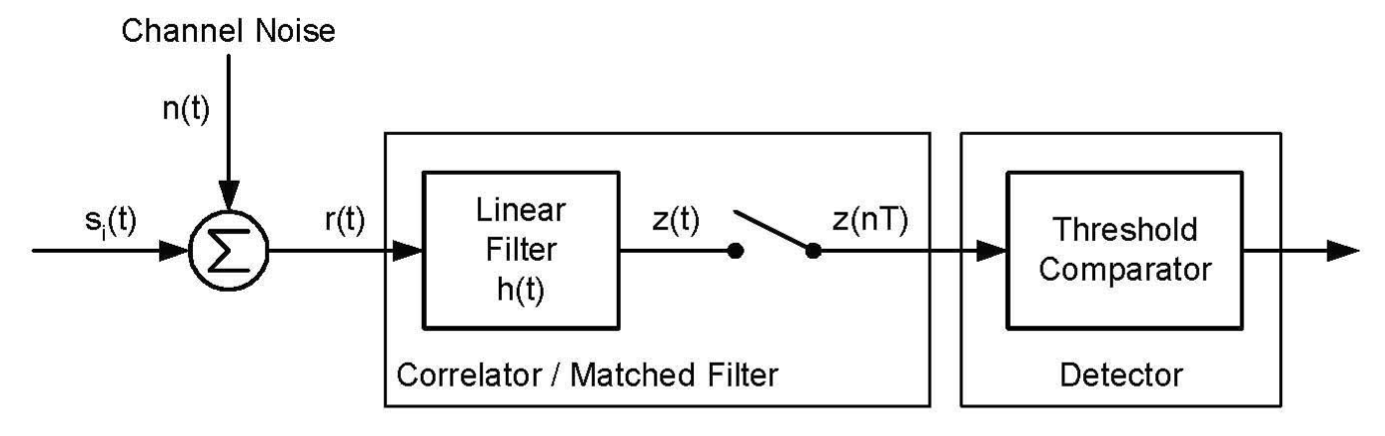
\includegraphics[width=9.5cm]{bilder/09_digital_signal_detection.png}
\end{minipage}
\begin{minipage}[c]{9cm}
	$$s_i(t) = \begin{cases}
          	s_1(t) & 0 \leq t \leq T \qquad \text{für Logisch } 1 \\
          	s_2(t) & 0 \leq t \leq T \qquad \text{für Logisch } 0          	
          \end{cases} $$
	$$\overset{Rauschen}{\Downarrow}$$
	$$	r(t) = s_i(t) + n(t) $$
	$$	\overset{Filter}{\Downarrow} $$ 
	$$	z(t) = r(t) \ast h(t) $$
\end{minipage}

\begin{enumerate}
  \item Am \textbf{Empfänger} $r(t)$ liegt das \textbf{Signal} $s(t)$ zusätzlich mit einem Additiven 
  		Weissen Gauss'schen (AWGN) \textbf{Rauschen} $n(t)$ vor.
  \item Mit dem \textbf{linearen Filter} wird das Signal-Rausch-Verhältnis (\textbf{SNR})
		\textbf{optimiert} (so \textbf{gross} wie möglich gemacht). Das Signal nach dem Filter sollte
		möglichst \textbf{wenig Rauschen} aber \textbf{viel Signalanteil} enthalten. \\
		Hierbei können zwei Strategien angewendet werden, das Matched Filter 
		\verweiskurz{09_matched_filter} oder der Korrelator
		\verweiskurz{09_korrelator}.
  \item Anschliessend wird das Signal \textbf{zeitdiskretisiert}, also immer nach einer konstanten Zeit
  		(Samplingzeit $t = T$) abgetastet. In der Praxis ist der opimale Abtastzeitpunktpunkt bei der maximalen SNR. Im Modell wird die SNR zum Zeitpunkt $nT$ maximiert. Dadurch resultiert: $z(nT) = a_i(nT) + n_o(nT)$, wobei $a_i(nT)$
  		dem Signalanteil und $n_o(nT)$ dem Rauschanteil entspricht. \\
  		Dies entspricht zwei Normalverteilungen, welche um die Mittelwerte ($a_1, a_2$) angeordnet sind.
  \item Schlussendlich wird mit dem Schwellwertdetektor entschieden, welches Signal
  		höchstwahrscheinlich gesendet wurde. Man unterscheidet die zwei verschiedenen Arten von
  		Detektoren: \\ \textbf{Hard-Decision:} Das Resultat des Detektors ist eine endgültige
  		Entscheidung (0 oder 1). Die Entscheidung wird mit Hilfe des Schwellwerts $\lambda_0$ gefällt.\\ 
  		\textbf{Soft-Decision:} Für 0 und 1 werden Wahrscheinlichkeiten bestimmt und verarbeitet.
\end{enumerate}

\subsection{Optimaler Detektor}
\subsubsection{Hypothesen und Fehlerwahrscheinlichkeit \schaum{227-9.2,3.A}}
	Für die Entscheidung existieren zwei \textbf{Hypothesen} ($H_1 \Rightarrow s_1$ wurde gesendet, 
	$H_2 \Rightarrow s_2$ wurde gesendet): \\ 
	Im binären Fall erfolt die Entscheidung mit einem Schwellwert $\lambda$: \qquad \parbox[c]{10cm}{
	Hypothese $H_1$ (falls $z(nT) > \lambda$): \quad $s_1$ wurde gesendet \\
	Hypothese $H_2$ (falls $z(nT) < \lambda$): \quad $s_2$ wurde gesendet}\\

\begin{minipage}[c]{10cm}
	\begin{center}
	 	\begin{tabular}{l l|c|c|}
	 		\cline{3-4} 
	 			& & \multicolumn{2}{c|}{empfangen} \\
			\cline{3-4}
				& & Mark = $H_1$ & Space = $H_2$ \\
			\hline
				 \multicolumn{1}{|l|}{\multirow{2}{*}{  gesendet }} 
				 & Mark = $s_1$, mit $P(s_1)$ & $\textcolor{green}{P(H_1 | s_1)}$ 
				 &  $\textcolor{red}{P(H_2 | s_1)}$\\
			\cline{2-4}
				\multicolumn{1}{|l|}{} & Space = $s_2$, mit $P(s_2)$ & $\textcolor{red}{P(H_1 | s_2)}$ 
				& $\textcolor{green}{P(H_2 | s_2)}$ \\
			\hline
		\end{tabular}  
  	\end{center}
\end{minipage}
\begin{minipage}[c]{8cm}
	Die \textbf{Fehler-WSK} $P_e$ ist somit wie folgt definiert:
	$$ P_e = \textcolor{red}{P(H_2 | s_1)} P(s_1) + \textcolor{red}{P(H_1 | s_2)}
	P(s_2)$$
\end{minipage} 

\subsubsection{Maximum Likelihood Detektor \schaum{227-9.3.B}}
Bei einem Maximum Likelihood Detektor ist der Schwellwert $\lambda_0$ genau so gewählt, dass die
\textbf{Fehler-WSK }$P_e$ \textbf{minimal} wird. \\
Konkret kann dies berechnet werden, indem man das \textbf{Minimum} von $P_e$ bestimmt, also: $\qquad
\dfrac{d P_e}{d \lambda_0} = 0 \qquad$ setzt. \\ 
Der Maximum Likelihood Detector entscheidet wie folgt: \qquad \parbox[c]{9cm}{Hypothese $H_1$: \quad falls $f(z|s_1)\cdot P(s_1) > f(z|s_2)\cdot P(s_2)$\\
Hypothese $H_2$: \quad falls $f(z|s_1)\cdot P(s_1) < f(z|s_2)\cdot P(s_2)$}\\

\begin{minipage}[c]{9.5cm}
 	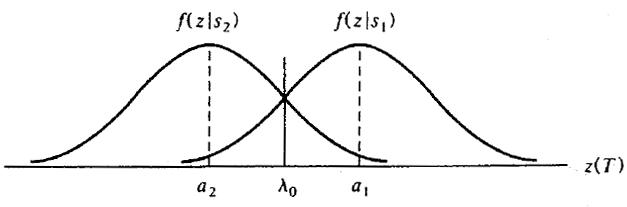
\includegraphics[width=8.5cm]{../NaT2/bilder/09_AWGN-PDF.png} \newline
 	$a_1 = $ Amplitude von $s_1 \cdot T$ \newline
 	$a_2 = $ Amplidude von $s_2 \cdot T$
\end{minipage}
\begin{minipage}[c]{7cm}
	 $$ \lambda_0 = \dfrac{1}{2} (a_1 + a_2) + \dfrac{\sigma_{n_0}^2}{a_1 - a_2}
 \ln\dfrac{P(s_2)}{P(s_1)} $$ 
 	$$ \lambda_0 = \dfrac{a_1 + a_2}{2} \qquad (\text{gilt für: } P(s_2) = P(s_1) = \dfrac{1}{2})
 	$$
 	$$ \text{mit } \sigma_{n_o}^2 = \frac{\eta \cdot T}{2}\text{, wenn weisses Rauschen}$$
\end{minipage} 

Somit beträgt die Fehler-WSK: $ \qquad P_e = \textcolor{red}{P(H_2 | s_1)} P(s_1) + \textcolor{red}{P(H_1 | s_2)}P(s_2) = 
 P(s_1) \int\limits_{-\infty}^{\lambda_0} f(z|s_1) dz + P(s_2) \int\limits_{\lambda_0}^{\infty}
 f(z|s_2) dz$ \\
Mit ($P(s_2) = P(s_1) = 0.5$) und ($\lambda_0 = \dfrac{a_1 + a_2}{2}$) gilt für ein
\textbf{NRZ-Signal}: $ \qquad P_e = Q \left(\dfrac{a_1 - a_2}{2 \sigma_{n_0}}\right) $



\subsection{Optimales Lineares Filter: Matched Filter \schaum{229-9.4.A}}
\label{09_matched_filter}
	\textbf{Ziel: } Maximierung von $(a_1 - a_2)$ bei gleichzeitiger Minimierung
	von $n_0$.
	%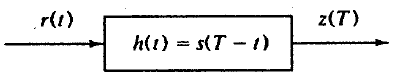
\includegraphics[width=4.5cm]{../NaT2/bilder/09_matched_filter.png}
 
	$$\text{SNR wird maximal bei } H \left( \omega \right) = S^* \left( \omega
	\right) \e^{-\jmath \omega T} \quad \IFT \quad h \left( t \right) = 
	\begin{cases} s(T-t) & 0 \leq t \leq T \\
	0 & sonst\end{cases}\text{ ; }h(t) = s(t) \text{, falls s(t) symmetrischer Puls}$$
	\begin{minipage}{6cm}{	
		$$ \left(\dfrac{S}{N}\right)_{0_{max}} = \dfrac{(a_1 - a_2)^2}{\sigma_{n_o}^2} = \dfrac{E_d}{\eta / 2} = \dfrac{2E_d}{\eta}$$} 	
	\end{minipage}
	\begin{minipage}{14cm}
		Mit $E_d$ als Energie des Differenzsignals $s(t) = s_1(t) - s_2(t)$ ; $ E_d = \int\limits_{0}^{T}[s_1(t) - s_2(t)]^2 \; dt$ \\
		
		Fehler- WSK des ML-Detektors: $P_e = Q\left(\frac{a_1 - a_2}{2\sigma_{n_o}}\right)  = Q\left(\sqrt{\frac{E_d}{2 \eta}} \right)$
	\end{minipage}
 	

\subsubsection{Variante zum Matched-Filter: Korrelator \schaum{230-9.4.B}} \label{09_korrelator}
Für den Sample Zeitpunkt ($t=T$) sind die Eigenschaften eines \textbf{Matched-Filter} und diejenigen eines
\textbf{Korrelators} \textbf{identisch}. Somit können beide für den selben Zweck eingesetzt werden.

$$ z(t) = r(t) \ast h(t) = \int_0^t r(\tau) h(t-\tau) d\tau \overbrace{=}^{h(t) =
h_{MatchedFilter}(t)} \int_0^t r(\tau) s[T - (t - \tau)] d\tau \overbrace{=}^{t = T} \underbrace{\int_0^T
r(\tau)s(\tau) \; d\tau}_{\text{Korrelator}}$$

	\begin{center}
		\begin{minipage}[c]{4.5cm}
			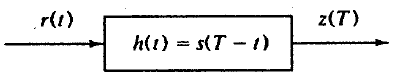
\includegraphics[width=4.5cm]{../NaT2/bilder/09_matched_filter.png}
			\centering Matched Filter
		\end{minipage}
		\begin{minipage}[c]{2cm}		
			$$\Longleftrightarrow $$
		\end{minipage}
		\begin{minipage}[c]{4.5cm}
			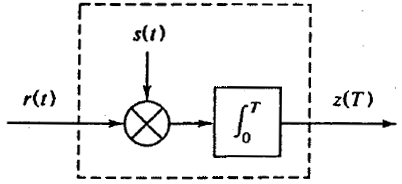
\includegraphics[width=4.5cm]{../NaT2/bilder/09_correlator.png}
			\centering Korrelator
		\end{minipage}
	\end{center}

\subsubsection{Unmatched RC-Filter \schaum{238-Prob.9.9}}
Hierbei wird an Stelle eines Matched Filters ein RC-Tiefpassfilter verwendet. \\
$$H(\omega) = \dfrac{1}{1 + j \omega R C} \qquad \qquad
 \left(\dfrac{S}{N}\right)_{0_{max}} = (0.815)\dfrac{2 A^2 T}{\eta}$$

\subsection{Fehlerwahrscheinlichkeit verschiedener binären
Übertragungen \schaum{231-9.5}}\label{09_binary_signals_error}
$E_b$ bezeichnet die mittlere Signalenergie pro Bit. Werte für Q-Funktion hinten im Schaum (S.326).

\renewcommand{\arraystretch}{2}
	\begin{tabular}{ p{6cm} p{2.5cm} p{9cm} }
		
		\multicolumn{3}{l}{\textbf{Allgemein optimaler Detektor}} \\
		$P_e= Q\left(\frac{a_1 - a_2}{2\sigma_{n_o}}\right)  = Q\left(\sqrt{\dfrac{E_d}{2\eta}}\right)$
		& \multicolumn{2}{l}{$E_d =$ Energie des Differenzsignals = $\int\limits_{0}^{T}[s_1(t) - s_2(t)]^2 \; dt$}
		\\
					
		\multicolumn{3}{l}{\textbf{Unipolar Baseband Signaling}} \\
		$ P_e = Q\left(\sqrt{\dfrac{A^2 T}{2 \eta}}\right) = Q\left(\sqrt{\dfrac{E_b}{\eta}}\right) $
		& $ E_b = \dfrac{A^2 T}{2} $
		& $ s_i(t) = \begin{cases}
		     s_1(t) = A & 0 \leq t \leq T \\       
		     s_2(t) = 0 & 0 \leq t \leq T
		   \end{cases}$ \\  

		\multicolumn{3}{l}{\textbf{Bipolar Baseband Signaling}} \\
		$ P_e = Q\left(\sqrt{\dfrac{2 A^2 T}{\eta}}\right) = Q\left(\sqrt{\dfrac{2 E_b}{\eta}}\right) $
		& $ E_b = A^2 T $
		& $ s_i(t) = \begin{cases}
 		     s_1(t) = +A & 0 \leq t \leq T \\       
 		     s_2(t) = -A & 0 \leq t \leq T
 		   \end{cases} $ \\

		\multicolumn{3}{l}{\textbf{Amplitude-Shift Keying}} \\
		$ P_e = Q\left(\sqrt{\dfrac{A^2 T}{4 \eta}}\right) = Q\left(\sqrt{\dfrac{E_b}{\eta}}\right) $
		& $ E_b = \dfrac{A^2 T}{4} $
		& $ s_i(t) = \begin{cases}
 		     s_1(t) = A \cos{\omega_c t} & 0 \leq t \leq T \\       
 		     s_2(t) = 0 & 0 \leq t \leq T
 		   \end{cases} $ \\

		\multicolumn{3}{l}{\textbf{Phase-Shift Keying}} \\
		$ P_e = Q\left(\sqrt{\dfrac{A^2 T}{\eta}}\right) = Q\left(\sqrt{\dfrac{2 E_b}{\eta}}\right)  $
		& $ E_b = \dfrac{A^2 T}{2} $
		& $ s_i(t) = \begin{cases}
 		     s_1(t) = A \cos{\omega_c t} & 0 \leq t \leq T \\       
 		     s_2(t) = A \cos{(\omega_c t + \pi)} = - A \cos{\omega_c t} & 0 \leq t \leq T
 		   \end{cases} $ \\

		\multicolumn{3}{l}{\textbf{Frequency-Shift Keying}} \\
		$ P_e = Q\left(\sqrt{\dfrac{A^2 T}{2 \eta}}\right) = Q\left(\sqrt{\dfrac{E_b}{\eta}}\right) $
		& $ E_b = \dfrac{A^2 T}{2} $
		& $ s_i(t) = \begin{cases}
 		     s_1(t) = A \cos{\omega_1 t} & 0 \leq t \leq T \\       
 		     s_2(t) = A \cos{\omega_2 t} & 0 \leq t \leq T
 		   \end{cases}$ \\

 	\end{tabular}
	\renewcommand{\arraystretch}{\arraystretchOriginal}
